\subsection{Bonita Intelligent Continuous Improvement (BICI)}


Bonita Intelligent Continuous Improvement ou \emph{BICI} fournit une solution pour soutenir la prise de décision dans le contexte de l'exécution du processus qui implique une conformité au \textit{SLA} (Service Level of Agreements).

Il est conçu pour aider les directeurs des opérations à s'assurer que l'exécution des processus qu'ils supervisent atteint des normes d'efficacité et, dans la mesure du possible.

Ceci est rendu possible par l'implémentation d'un algorithme d'exploration de processus, qui utilise à la fois l'horodatage (timestamp) de tous les événements BPM et l'identifiant de chaque instance de processus dans les archives Bonita pour construire le chemin fait par chaque cas et son historique.

BICI a trois parties. Voir Figure \ref{fig:ici_architecture}
\begin{itemize}
  \item Serveur. Le serveur principal interroge les données, crée des modèles d'exploration de processus et sert les API REST.
  \item Stockage. Il stocke les données ICI et les modèles prédictifs, et il s'appuie sur le moteur Elasticsearch.
  \item Configuration de la Living App. Il est utilisée pour configurer les processus
  \item Opération d'Administration. Il est utilisé pour afficher les informations d'exécution de cas et les prédictions pour les gestionnaires d'opérations.
\end{itemize}

\begin{figure}[!ht]
\centering
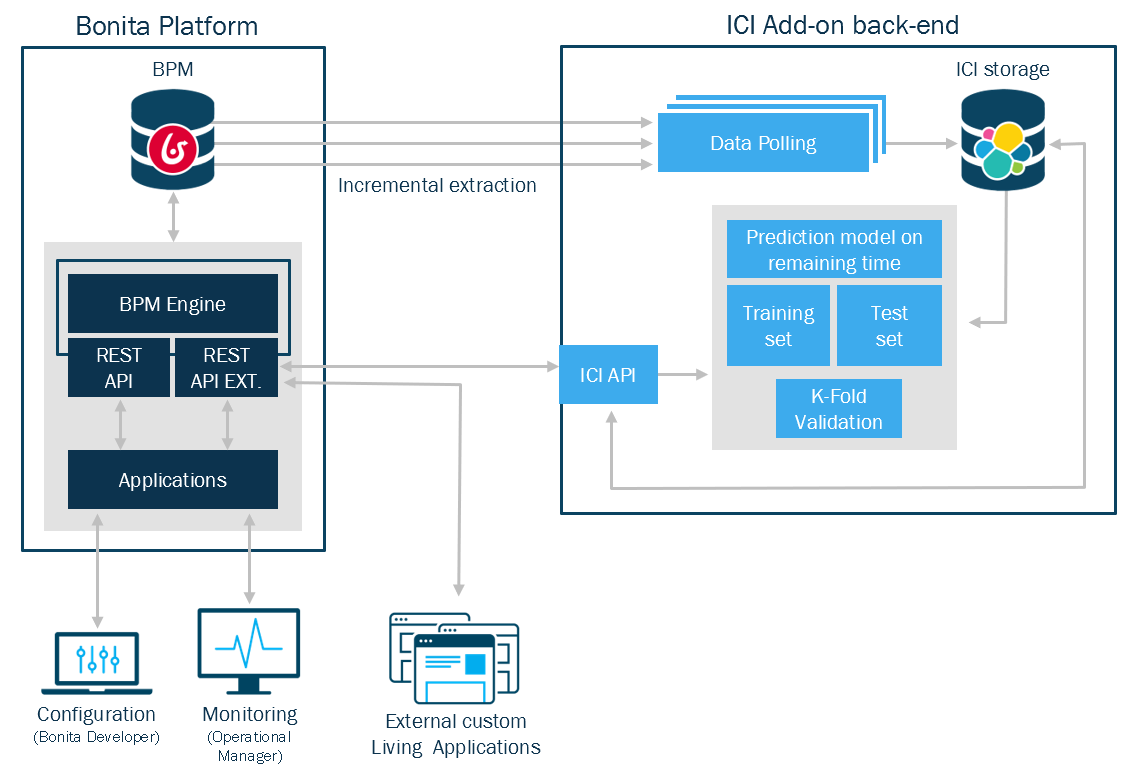
\includegraphics[width=\textwidth,keepaspectratio]{ici_architecture.png}
\caption{BICI Architecture}
\label{fig:ici_architecture}
\end{figure}
